
\def\FunctionF(#1){(#1)^3- 3*(#1)}%
\def\FunctionFPrime(#1){3*(#1)^2- 3}%

\begin{frame}
\begin{center}
	$\mathcal{OUTILS\,\,\, MATHEMATIQUES}$
\end{center}
\end{frame}

\subsection{D�rivation}
\begin{frame}
\frametitle{D�rivation}
\begin{tabular}{c  c}
Graphe de la fonction & \only<2,3,4,5>{D�riv�e de $f$:}\\[2mm]
$f:
\left\{
	\begin{array}{ll}
		\R \to \R\\
		x\mapsto x^3-3x
	\end{array}
\right.$ & \visible<2,3,4,5>{$f':
\left\{
	\begin{array}{ll}
		\R \to \R\\
		x\mapsto\only<2,3,4>{?}\visible<5>{3x^2-3}\only<5>{\visible<4>{?}}
	\end{array}
\right.$}\\[4mm]
\begin{minipage}{5cm}
\begin{tikzpicture}[scale=0.5]
\begin{axis}[
        axis y line=center,
        axis x line=middle, 
        axis on top=true,
        xmin=-5.5,
        xmax=5.5,
        ymin=-45,
        ymax=45,
        height=12.0cm,
        width=12.0cm,
        grid,
        xtick={-5,...,5},
        ytick={-40,-32,...,40},
    ]
    \addplot [domain=-5:5, samples=50, mark=none, ultra thick, blue] {\FunctionF(x)};
    \node [left, blue] at (axis cs: 3.6,42) {$x^3-3x$};
\end{axis}
\end{tikzpicture}
\end{minipage}&%
\begin{minipage}{5.5cm}
\begin{center}
\only<1,2,3,4>{
\visible<3,4>{\textit{D�finition :} pour $x\in\R,$
$$f'(x) := \lim_{h\to0}\frac{f(x+h)-f(x)}{h}$$}
\visible<4>{\textit{Propri�t� :} soient $f$ et $g$ deux fonctions d�rivables, $a, b\in\R, n\in\N^*$. Alors\\ [1mm]
$(a f + b g)' = a f' + b g'$\\[1mm]
$(fg)' = f'*g + f*g'$\\[1mm]
$(f^n)' = n(f')f^{n-1}$}
}
\only<5>{{
\begin{tikzpicture}[scale=0.5]
\begin{axis}[
        axis y line=center,
        axis x line=middle, 
        axis on top=true,
        xmin=-5.5,
        xmax=5.5,
        ymin=-45,
        ymax=45,
        height=12.0cm,
        width=12.0cm,
        grid,
        xtick={-5,...,5},
        ytick={-40,-32,...,40},
    ]
    \addplot [domain=-5:5, samples=50, mark=none, ultra thick, red] {\FunctionFPrime(x)};
    \node [left, red] at (axis cs: 3.6,42) {$3x^2-3$};
\end{axis}
\end{tikzpicture}}}
\end{center}
\end{minipage}
\end{tabular}
\end{frame}

\subsection{Equations diff�rentielles}
\begin{frame}
\frametitle{Equations diff�rentielles}
\begin{center}
\'Equation dont l'inconnue est une fonction $f$,  entre $f$ et ses d�riv�es.\\
\visible<2,3,4>{Exemples :}
\visible<2>{$f'(x)=f(x)$}
\visible<3>{$f' = f^2-3f+2$}
\visible<4>{$f'(x) +f''(x) = \frac{f^2(x) + 1}{1+x^2} $}
\visible<5,6,7,8>{Existence et unicit� d'une solution ?}\\
\visible<6,7,8>{Pr�ciser des conditions aux limites.}\\
\visible<7,8>{Trouver le domaine.}\\[6mm]
\visible<8>{De nombreux th�or�mes (Lipshitz), de nombreuses conjectures.}
\end{center}
\end{frame}

\begin{frame}
\frametitle{Equations diff�rentielles}
\visible<1>{Comment tracer les solutions ?}\\[3mm]
\visible<2,3,4>{R�solution \underline{graphique} de 
$\left\{
	\begin{array}{ll}
		f' = f \\
		f(0) = 1.
	\end{array}
\right.$}
\begin{center}
\begin{tikzpicture}[scale=0.5]
\begin{axis}[
        axis y line=center,
        axis x line=middle, 
        axis on top=true,
        xmin=-5,
        xmax=5,
        ymin=-1,
        ymax=10,
        height=12.0cm,
        width=12.0cm,
        grid,
        xtick={-5,...,5},
        ytick={-1,0,...,10},
    ]

\only<3>{\addplot[ samples=41, mark=*, blue]{exp(x)};}
\only<4>{\addplot[ samples=61, mark=none, blue]{exp(x)};}
\end{axis}
\end{tikzpicture}
\end{center}
\end{frame}

\begin{frame}	
\frametitle{Equations diff�rentielles}
\begin{center}
\includegraphics[width=11cm]{EquaDiff.jpg}
\end{center}
\end{frame}

\subsection{Al�atoire}
\begin{frame}
\frametitle{Mouvement brownien}
\begin{center}
\begin{tabular}{c c c}
 1827&1905&1921\\[1mm]
 \hline\\ [-1.8ex]
 \visible<2,3,4>{Biologie}&\visible<3,4>{Physique}&\visible<4>{Math�matiques}\\[1mm]
 \hline \\ [-1.5ex]
 \begin{minipage}{3.0cm}
  \visible<2,3,4>{\footnotesize{\textbf{Robert Brown} remarque au microscope que le mouvement de grains de pollen sur l'eau ne suit pas de logique �vidente.}}
 \end{minipage}
 &
  \begin{minipage}{3.0cm}
  \visible<3,4>{\footnotesize{\textbf{Albert Einstein} publie une th�orie quantitative du mouvement brownien.}}\end{minipage}
  &
   \begin{minipage}{3.1cm}
 \visible<4>{  \footnotesize{\textbf{Norbert Wiener} propose un cadre formel au mouvement brownien\,: le processus de Wiener.}}\end{minipage}
\end{tabular}
\end{center}
\end{frame}

\begin{frame}
\frametitle{Mouvement brownien}
\begin{center}
\includegraphics[width=11cm]{MvtBr.jpg}
\end{center}
\end{frame}

\begin{frame}
\frametitle{Mouvement brownien}
Permet une th�orie du calcul stochastique \\(des �quations diff�rentielles qui contiennent de l'al�a)\\
\visible<1,2,3,4>{$$f'(t) = -f(t) \,\textcolor{gray}{\to}\, \visible<2,3,4>{\frac{\text{d}f}{\dt}(t) = -f(t)}\,\textcolor{gray}{\to}\,  {\footnotesize\visible<3,4>{\frac{\text{d}f}{\dt} = -f} \,\textcolor{gray}{\to}\, \visible<4>{\text{d}f = -f\, \dt}} $$}
\visible<5,6>{
\begin{tabular}{l l}
Calcul classique : &$\text{d}f = -f\, \dt$\\
\visible<6>{Calcul stochastique : }&\visible<6>{$\text{d}f = -f\, \dt+\text{d}B_t$}
\end{tabular}
 }
\end{frame}